


\chapter[*Advanced Agentic Architectures]{*Advanced Transformer and Agentic Architectures}\label{chap:arch}

\begin{learningbox}
In this chapter you will learn about advanced transformer and agentic architectures. Specifically, you 
will be able to:
\begin{itemize}[leftmargin=*, nosep]
    \item Understand the concept of {\em Turing-completeness}, and learn that transformers are, in principle, Turing-complete.
    \item Understand that transformer models can perform planning, when we train them on {\em decision traces}, instead of on natural language. 
    \item Describe how embeddings can be connected directly to other embeddings, in {\em looped language models}, skipping tokenization layers. 
    \item Describe how agents can perform {\em reinforcement learning in-context}, by storing a history of state-action-reward triples.
    \item Describe the advantages and disadvantages of {\em self-modifying} agents. 
    \item Understand how metalearning can be applied to harness design, to create a {\em meta-harness} that improves the basic harness.
\end{itemize}
\end{learningbox}

\section{Transformer Architectures}
The success of large language models has spawned interesting new research avenues into transformer architectures. LLMs were good at language, but not at other problem types such as reasoning and planning. This caused researchers to explore the limits of the types of computations that transformers were able to do, and we will discuss some of the topics in the following sections. Specifically, they asked the questions whether transformers were Turing complete (Section~\ref{sec:turing})? The weak performance on planning problems prompted studies that trained transformers directly on decision traces, to see if that allowed them to be able to plan and backtrack (Section~\ref{sec:decisions}). Next, we will look at looped language models, where multiple models are connected directly at the level of the embeddings. 


\subsection{Transformers are Turing-complete}\label{sec:turing}
The difficulty of LLMs to manage state at inference time suggests that LLMs are limited in the type of computations that they can perform. %What types of computations are transformers able to perform? %Associative next-word prediction: yes, state: no.
In theoretical computer science the concept of Turing completeness indicates whether a certain model of computation is powerful enough to be able to perform any type of computation of a certain category (which includes being able to manage state values correctly). This concept was introduced in a famous paper by Alan Turing in 1936, in which he proved that a certain type of machine would be powerful enough to do so \citep{turing1936computable}. 
To be called Turing complete, a system must be able to simulate any other computational device and be able to process any problem that can be expressed in an algorithm (but perhaps take infinite time and memory to do so). 
%In theory, a certain type of machine, the Turing machine, is capable of general computations. The Turing machine is a simple machine, consisting of a tape, a read/write head, and a memory. 
It turns out that it is not too difficult to achieve  Turing completeness; most general purpose programming languages are Turing complete.\footnote{For example, the Python programming language is Turing complete, but simple regular expression matching, without backreferencing, is not.} 

The difficulty of LLMs---and of transformer-based models in general---to manage state would suggest that the transformer architecture may not be Turing complete. 
Interestingly, already in 2021 \citet{perez2021attention} have studied this question, and have proven that the transformer architecture is able to simulate a Turing machine, and is thus Turing complete.

This is an encouraging result, since it indicates that there is no fundamental reason why transformers would not be able to manage state correctly. It may well  be a matter of finding the right prompt, or finding the right pretraining and finetuning dataset. 

Unfortunately, the fact that something is theoretically possible, does not mean that achieving it will be easy, or that it can be done efficiently. %It may be that they must be heavily finetuned to efficiently perform certain computations. 
For example, it might be that certain architectural extensions to the transformer architecture  would enhance the ease with which efficient state management can be achieved. 
We will now discuss methods that have been developed so that LLMs can efficiently solve  decision making and planning problems.


\subsection{Pretraining Backtracking on Decision Traces}\label{sec:decisions}
%\todo{delete? Goes too far? Mwa, misschien toch houden, want het idee dat je alles kunt bereiken als je er maar op traint is een krachtig idee. En wat we natuurlijk graag willen is dat ook general-language-trained LLM het kunnen. Dat is een uitdaging, dus daar gaan de andere subsecties dus over. Deze gedachte moet ik in de tekst stoppen.
The finding that transformers are Turing-complete encourages research in planning and decision making. 
%It suggests that we only need to find a way to train or query the model in the right way in order to be able to make a decision. 
In this section we will discuss studies that pretrain a transformer architecture on decision traces, to good results. Note that this section is {\em not} about transformers that are trained on natural language---LLMs---but on transformers trained on decision traces. %In  section~\ref{sec:inferencetime} we will discuss studies that use transformers trained on natural language with inference-time methods.

\begin{figure}
    \centering
    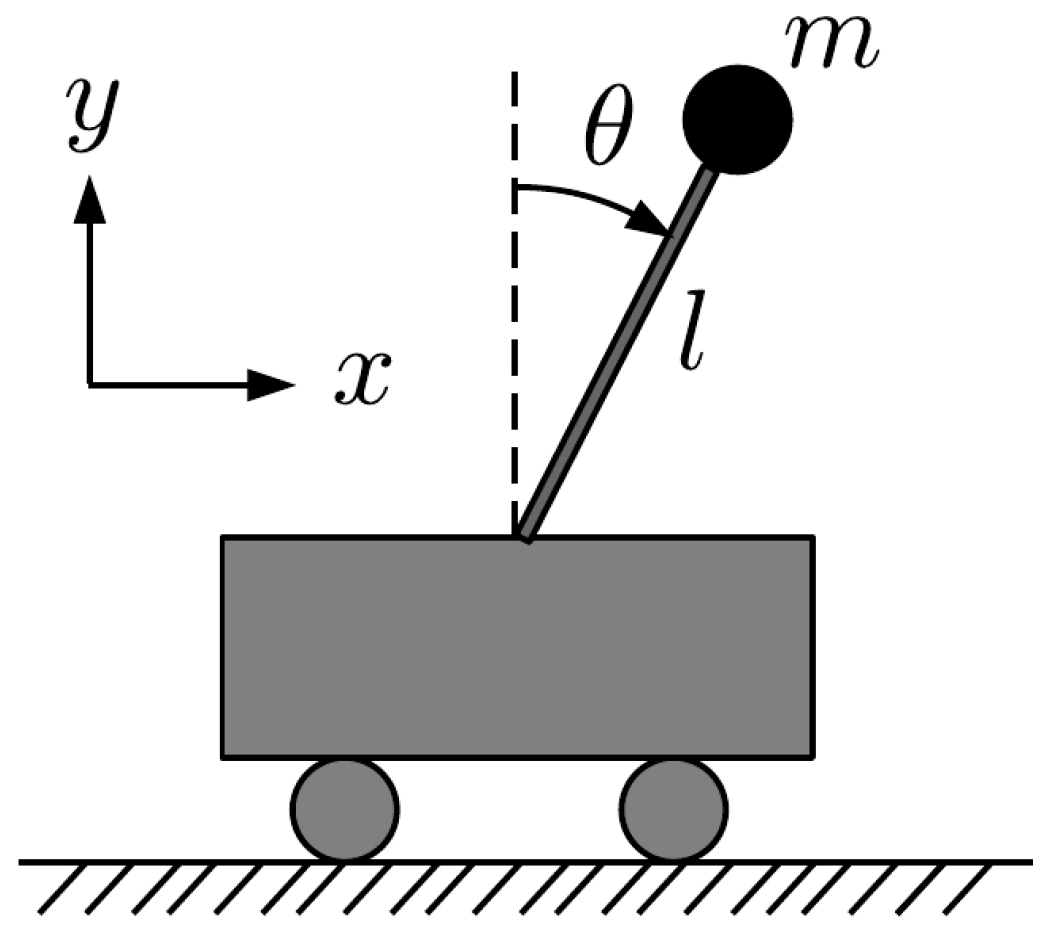
\includegraphics[width=0.5\linewidth]{figures/cartpole}
    \caption{The Cartpole Problem: Balance the Pole just by Moving the Cart Left or Right}
    \label{fig:cartpole}
\end{figure}

%To see if transformers can perform planning and decision problems, 
First we discuss pretraining transformers directly on decision traces: sequences of state-action-reward triples, {\em not} language tokens. %, instead of first on natural language. 
%The reinforcement learning approaches that we discussed so far---React, Self Refine, Tree of Thoughts,  Reflexion---use external algorithms to manage state for the prompt improvement loop. A perhaps more elegant solution would be to perform reinforcement learning fully in-context, within-prompt. 
%!!!!!!!!!!!!!!!!!!!! In agentic LLM our agents must be able to make decisions, act in the world, and learn from the consequences of those decisions. The question whether transformers are suitable for decision making has been studied widely. Specifically, 
Several works study whether transformer networks can be trained to perform reinforcement learning---to learn from feedback, to perform learned policies, and to explore to learn better actions. \citet{chen2021decision,lee2023supervised,wang2024transformers}  showed that  basic transformer architectures can indeed be pretrained and finetuned on decision  traces from typical planning problems. %These studies showed that at test-time, transformers perform reinforcement learning, in-context. 
When an empty (non-language trained) transformer is pretrained on decision traces, it can exhibit in-context reinforcement learning (ICRL). So far, this has been shown using toy problems such as Boyan's chain and Cartpole (see Figure~\ref{fig:cartpole}).  
Furthermore, in the games of Chess and Hex encouraging results were achieved by pretraining the decision transformer on minimax \citep{markeeva2024clrs,knuth1975analysis} and MCTS \citep{browne2012survey} search traces \citep{schultz2024mastering,kempinski2025game}. Transformers were able to learn to lookahead and search a few steps. Other works report encouraging results in the game of Othello \citep{li2023emergent,kempinski2025game,chen2025if}. 

A further work that studies how transformer architectures can be trained to perform decisions is {\em self backtracking} \citep{yang2026step}. In this approach the model is again trained on decision traces. However,  a new kind of token is introduced, $<$backtrack$>$, that prompts the model to perform explicit backtracking at inference time. The model is trained on a dataset of decisions, and when an error is encountered during training, the $<$backtrack$>$ token is learned, to find an alternative solution. At inference time, then, this backtracking is performed. A mechanism that consists of expansion/backtracking/selection is executed by the model, so that alternative solutions for the state in question are examined. 

The self backtracking approach reports good results on typical planning problems such as the 24-game and maze navigation, compared to standard baselines on small versions of DeepSeek-R1 and Qwen3. Through the introduction of a new type of token and new backtracking-functionality in the model, this approach allows enhanced-transformer models to perform search, blurring the line between training and inference.

These are encouraging results, although it is still an open question to what extend the weakness of transformers in managing state has been solved. Performing inference-time ICRL on larger problems is an area of active research. 

%In addition to planning, agents should have memory. The question of how to provide agents with suitable types of memory is an area of active research, see also Section~\ref{sec:memory}.

\subsection{LoopedLLM and Recursive Multi-Agent Systems}
Improving the  expressive power of transformers brings them closer to a general purpose programming architecture. We will discuss two other  developments: looped language models and recursive systems.

It is easy to connect LLM agents at the language level: just let them speak to each other in natural language, on which they are all trained. However, this necessitates many (de)tokenization steps, which take time and introduces differences between embeddings. Can we directly connect embeddings, bypassing the tokenizers, and do training and inference at that level?


\citet{giannou2023looped}
show  how %programs written in Restricted Access Sequence Processing language  can be mapped onto transformer networks. They show how
looped transformers (transformers whose input neurons are directly connected to transformer
output neurons, either from the same or from another model) can emulate a basic
calculator, a basic linear algebra library, and in-context learning
algorithms that employ backpropagation. Looped transformers are a powerful architecture, see for example \citet{yang2023looped,saunshi2025reasoning,zhu2025scaling}.

A further development of direct embedding-to-embedding connections is recursive multi-agent systems \citep{yang2026recursive}. This approach  connects heterogeneous
agents in a collaboration loop, enabling in-distribution
latent thought generation and cross-agent latent state transfer. An inner-outer loop learning algorithm (metalearning, see Chapter~\ref{chap:meta}) performs  whole-system co-optimization through shared
gradient-based credit assignment across recursion rounds. Experiments with four agents over  benchmarks from mathematics,
science, medicine, search, and code generation, showed stable multi-agent training. In comparison with other single/multi-agent and
recursive  baselines, accuracy is improved by a few percentage points, inference is twice as fast, and token usage is  reduced by  comparable ratio. 

An innovation of RecursiveMAS is the introduction of a two-level recursive-link. Training a multi-agent system is  difficult because gradients must flow through multiple models, and this process can become unstable. RecursiveMAS improves this process by freezing the parameters of the underlying LLMs and only training the lightweight RecursiveLink modules. The training occurs in two stages.

%Recursive and LoopedLLMs are recent developments that hold much promise. 

\section{Agentic Architectures}
In addition to new transformer architectures, the work on agentic LLMs has also led to advanced agentic architectures. First, we will look at in-context  reinforcement learning, where we will see that LLMs are able to perform policy improvement when the prompt is given a history of state-action-reward triples. Second, we will look at self-modifying agents, and discuss the advantages and disadvantages of this approach. Finally, we will look at meta agents.



\begin{figure}
  \begin{center}
    \input figures/rl
    \caption{For reference, the standard reinforcement learning loop where the agent learns a $\theta$-parameterized policy $\pi_\theta$ from feedback rewards $r$ from the environment upon its actions $a$, selected from policy $\pi_\theta$, etc. \citep{sutton2018reinforcement}}\label{fig:rl6}
  \end{center}
\end{figure}


\subsection{In-Context Reinforcement Learning}\label{sec:icrl}
%\subsubsection{Learning-based Prompt Optimization}\todo{Merge with ICRL section???}
Recall from Section~\ref{sec:rl} that the goal of reinforcement learning is to compute a  policy that has an optimal action  for each state \citep{sutton2018reinforcement}. 
As the agent converges towards this policy, in each timestep, the agent learns these actions from feedback from its environment, the rewards.  
These rewards reinforce the confidence of the agent in the policy's actions in each state (see Figure~\ref{fig:rl6}). %\
The self-reflection approaches from the previous section borrow  many ideas from reinforcement learning for the agentic harness. We will now discuss related methods that optimize prompts by  in-context reinforcement learning, where the LLM performs prompt improvement.



%\todo{Wat i nu eigenlijk de boodschap van deze sectie? Dat ICRL bestaat? Of wat? Merge 6.2.3.5 and 6.2.3.7???}
%, in these  approaches the external self-reflective prompt improvers play the role of agent tyring to find the optimal policy, and the LLM provides the feedback as environment. 

%In Section~\ref{sec:decisions} we saw that transformers, when trained on decisions, exhibit reinforcement learning behavior such as temporal difference learning. In the previous section we saw that external prompt optimizers can exhibit reinforcement learning on on transformers that are trained on natural language. Approaches such as ReAct, Reflexion and Buffer of Thoughts use an external memory to manage the prompt invocations. They use a self-reflection loop to find an optimal prompt for the LLM, just as a  reinforcement learning agent optimizes its policy using feedback from its environment (the LLM). 

%Interestingly---or perhaps confusingly---
Reinforcement-type learning mechanisms  have  been observed to emerge directly in LLMs, when environment histories were provided to the LLM by an external prompt optimizer: the LLM in certain self-reflection loops can perform policy-improvement. This phenomenon is called  in-context reinforcement learning (ICRL) \citep{song2025reward}, see Figure~\ref{fig:rl-icrl}. %(Do not be confused. Whereas in the previous section the LLM was the {\em environment} providing  feedback to the prompt optimizer harness, in this section the LLM is the {\em agent} optimizing the policy, see Figure~\ref{fig:rl6}. In Section~\ref{sec:styles}, we will elaborate on different agentic learning styles.)


\citet{krishnamurthy2024can}  asked the question whether generic LLMs that are trained on language can explore in-context, and whether they can learn in-context from feedback. This question  has since been answered positively by various studies \citep{demircan2024sparse,song2025reward,moeini2025survey,monea2024llms,nie2024evolve,wang2024transformers}. %\todo{So we should delete the krishnamurthy question?} 

%To use reinforcement learning as a prompt optimizer for LLM, 
In ICRL,  an external harness  iteratively calls the LLM, feeding it a sequence of action, state, and reward triples, in-context (Figure~\ref{fig:rl-icrl}). The history of triples grows in each iteration. The LLM reacts by improving its implicit policy, providing increasingly good action choices in each iteration, thus we conclude that it performs the essence of reinforcement learning inside the LLM. 

In ICRL, %the reasoning problem is formulated as a Markov decision process: 
the agent-algorithm selects an {\em action}, to sample a step  and get an answer (a {\em state}, {\em reward} pair) from the environment, see Figure~\ref{fig:rl-icrl}. A Markov decision process, or MDP, is a process in which all relevant information to calculate the next state is contained in the previous state and the action taken. Therefore, the prompt for the policy-LLM contains  all relevant information, it accumulates the history of $(s,a,r)$-triples, which the LLM can use to improve the policy of the best action for each state.
\begin{figure}[t]
  \begin{center}
    \input figures/rl-icrl
    \caption{ICRL: Prompt Optimization with Reinforcement Learning}\label{fig:rl-icrl}
  \end{center}
\end{figure}
For state, the  history of answers is a natural choice, but, in general, how to best model LLM prompt improvement as an MDP is still an active area of research.

In ICRL the agent uses the LLM for the policy-function. The LLM can also be used (with a different prompt) to play the role of environment, as in a self-reflection harness.

In-context reinforcement learning
%Abstract: RL emerges in LLM's (Large Language Model) inference time---a phenomenon known as in-context RL (ICRL). Specifically, we propose a novel 
occurs in a multi-round prompting harness, % called ICRL prompting. The goal is to prompt the LLM to complete a task. 
where, after the environment-LLM generates a response at the current round, a numerical reward is calculated by the LLM for the response that the LLM just calculated. %scalar feedbacks for the response, called the rewards. 
At the next round, the agent-LLM is prompted again with the same task and a context that now consists of the previous responses and rewards. The % In their experiments, the authors found that  the 
quality of the agent-LLM's response increases as the context becomes longer. 
Just like a reinforcement learning algorithm, the LLM is able to maximize the numeric reward, at inference time. \citet{song2025reward} report how the ICRL approach was validated on the applications of tree of thoughts %(, just like an RL algorithm. We evaluate ICRL prompting in three benchmarks 
(Game of 24, creative writing, and ScienceWorld), outperforming %. and demonstrate significant performance improvements over baseline methods such as 
self refine and reflexion. %Surprisingly, in some experiments the reward signals are generated by the LLM itself, yet performance improvements are still observed from ICRL prompting, offering a promising paradigm for scaling test-time compute .
%This\todo{Hmm} is also the goal of the Algorithm of Thoughts (AoT) approach \citep{sel2023algorithm}, which aims to learn algorithms in  context in general LLMs such as GPT-4, Claude and Gemini 1.5. They achieve results comparable to Tree of Thoughts on GSM8K, StrategyQA, and Crosswords. Achieving these results with in-context reinforcement learning is a promising result for in context learning. %Other search-like in-context algorithms are studied by \citet{schultz2024mastering} and \citet{kempinski2025game} (Game of Thoughts). %Further work in games finds that LLMs struggle with the knowing-doing gap and the difference between using and mentioning game concepts \citep{paglieri2024balrog,van2025baba,cloos2024baba}.  
%


How does the ICRL process work, inside the LLM? At
%\todo{How does ICRL work?} 
inference time the LLM performs a forward pass through the transformer network, computing the inference token. This forward pass has been found to    
%focuses on the ability of the forward (inference) pass to 
implicitly perform reinforcement learning \citep{wang2024transformers}. 
%
\begin{comment}
In ICRL, in each iteration $(s,a,r)$ feedback tuples are added to the context. As this history grows, 
%They wrote: {\em Notably, the context can span multiple episodes. As the context length increases, 
action quality improves. \citet{wang2024transformers} find that this improvement is not due to memorized policies encoded in the fixed parameters but that a reinforcement learning process occurs during this forward pass as the agent processes the context.
\end{comment}
%
%Note  that the principle of reinforcement learning is that the agent tries to learn the world by sampling only. Using the same LLM by the environment and by the agent breaks the strict separation between agent and environment. No no no. What is the environment? This is all in context RL. The environment is the context of the LLM. Using the same LLM for action selection (by the agent ) and for action evaluation (by the environment) is cheating, it would make it easy for the agent to select good actions. No it is not. It is dynamic programming. The only goal is to select good prompts, good actions. to get the best out of the LLM. Simple optimization. Might as well use EA. Why are we doing RL? Is it parameterized? How is the policy represented? Just a history for an LLM? Very loose mapping of states to actions. There is no Q-learning. It is dynamic programming, or random search, without gradients. Just let the LLM generate the next action and hope it does it smart. No DQN, REINFORCE, Q-learning. just ask the LLM. And notice that the LLM process performs reward optimization. So inside the LLM there is an RL optimization process going on, when we provide a loop of prompts for it. 
In other words, 
in-weights learning is where the model has learned the right answer from its trained weights, at training time;
in-context learning is where the model has learned the right answer at inference time from few-shot examples provided in its context; and
in-context reinforcement learning is where the LLM has learned the right answer using (apparent) reinforcement learning on a growing sequence of the state-action-reward triples that it produced itself through inference. Thus, the reinforcing algorithm, optimizing the policy, is done implicitly by the LLM forward pass (inference step) when a sequence of prompts or history is given in the context. 


Note that the LLM can be used for the agent, as a policy optimizer, and for the environment, to calculate the next state and reward. To ensure that the agent is learning without accidentally benefiting from the environment's knowledge, it is better to use a separate LLM. This, too, is an active area of research.

\begin{comment}
    
\paragraph{In-Context Reinforcement Learning}\todo{Naar hoofdstuk 6, 6.2.4.3 ICRL?}
The bottom of the figure shows the in-context reinforcement learning approach. The evaluation-LLM plays the role of the environment, and generates the new state and the reward value \citep{moeini2025survey}. The policy-LLM plays the role of the agent which generates the actions. The agent accumulates the state, reward, and action values to form a history, which is given as prompt to the LLM, that computes the new action. In reinforcement learning terms, the LLM uses the history-prompt to perform policy-improvement, selecting the best action to go with the new state that it received from the environment. When the model provides increasingly better actions with the growing prompt, policy improvement is occurring, and the model is said to perform in-context reinforcement learning (ICRL) \citep{laskin2022context,lu2023structured}. 

Note that the history grows in length with each iteration of the reinforcement learning loop, as the $(s,a,r)$ tuples are added. In most LLMs the size of the context window limits the number of iterations that are possible. For this reason history compression methods are introduced, or special long-context window LLMs can be used. This is an active area of research \citep{liu2025comprehensive,fei2024extending,sheng2025dynamic}.

Note that in this interaction style, we have  entered the situation where LLMs generate prompts
to be evaluated by that same LLM. LLMs are self-reflecting on their own
results. Self-reflection may work when we assume that it is easier to evaluate the quality of existing
results than that it is to create a good result. Self-reflection is not guaranteed to work, as the chapter on metalearning highlighted. It is also possible
that the self-reflective series of self-calls degenerates, and that
the setup does not work at all. For a situation where clear evaluation
criteria exist, such as when code is generated and an external
interpreter can check correctness, self-reflection has a higher chance
to work. When the evaluation is noisy, it may not.


The tree of thoughts \citep{yao2024tree} approach and the  React \citep{yao2022react}, reflexion \citep{shinn2024reflexion} and self refine \citep{madaan2023self} approaches are prominent examples of these self-reflective in-context learning approaches.  Examples of the prompt sequences have been given in Section~\ref{sec:reflective} in Chapter~\ref{chap:reasoning}.

\end{comment}

%In contrast to the external self-reflection approaches, in ICRL there is no explicit Q-learning being done outside the LLM
%So self-reflection using the same LLM for evaluation and generation, as ToT does, should work, it is like Dynamic Programming, just a way to find the best policy in an LLM. Dat is niet erg, want het is een supervised setup, ToT learns a policy die dan tegen een benchmakr gebruitk wordt. ToT en CoT gaan allemaal tegen benchmarks. Al de RL approaches en self reflection approaches are created to get good answers from the LLM. So the pictures are all wrong. The benchmark should be the environment that they are testing against. Figure 8.5 (D) is wrong, there is no theta parametering the policy. The policy is the LLM, which has the parameters. Parameterized by the transformer weights, and by the context (prompt). There are two LLM instances, a policy and an evaluator. The loop is good, but the word Environment must be deleted.


%% %\paragraph{Auto-GPT}
%% Auto-GPT. Just some combination of other ideas and a lot of publicity. In a way that does not
%% work.
%% Can be used as negative example of too much halucination, too
%% difficult to incorporate outside knowledge, too much self-guiding
%% leads to feedback loop.
%% Whatch out for feedback loops.

\subsection{Self-Modifying Hyperagents}
In this book, we have discussed self-reflective prompt improvers that are based on search algorithms and  reinforcement learning. The code for these external algorithms is written by human researchers, and does not change as the agent is learning. The approach by which the prompt is improved is limited by these static algorithms.

LLMs excel at manipulating and judging computer code \citep{zhuge2024agent}. We could, in principle, easily ask them to generate code for an agentic prompt harness, or for an in-context reinforcement learning harness. We could even ask the LLM to run the code on a particular problem instance, and, based on the outcome of the experiment, ask for an improvement of the prompt-improver code.
If the LLM is good at using experiment-results for writing prompt-improvement code, this approach could work better than  standard approaches from the published literature.

Self-modifying code (computer programs that alter their own instructions while they are being executed) has a long history in computer science \citep{cai2007certified}, as an alternative to conditional branching statements. Many computer languages support it, from  assembly languages, to Lisp \citep{abelson2022structure} and Python. It is a powerful method that can be used for performance improvement, for example in just-in-time compilation \citep{ansel2011language}. However, programs become less predictable, which may cause problems in finding errors in the program, and raises security concerns. For this reason the use is sometimes discouraged when predictability of  programs is important.  

An advantage of self-modifying agents is open-endedness: they can  continuously improve themselves, without fixed boundaries set by static algorithms \citep{schmidhuber2007godel}. A challenge is to do this safely \citep{zhang2026darwingodelmachineopenended}.  
In Darwin-G\"odel-Machine-Hyperagents the authors  integrate (1) an agent to solve the target task with (2) a meta agent to  modify itself and the task agent, into a single (editable) program. Note that the meta-level modification procedure is itself editable, enabling self-modification. This allows, in principle, not only improving the task-solving behavior, but also the mechanism that generates future improvements \citep{zhang2026hyperagents}. The experiments, however, do not  achieve full openness, as they use a fixed task distribution, as well as fixed parent selection and evaluation protocols. 

As approaches become more open-ended, paradoxically, a challenge becomes to control the process of improvement, to ensure that it does not degenerate, but keeps improving \citep{cemri2025multi,ecoffet2020open}. 
In general, the problem of powerful metalearning approaches is to ensure stable learning processes. Powerful generation requires powerful evaluation---adaptation to fit the environment. %Chapter~\ref{chap:meta} discusses this problem further, but we first switch to another approach.

\subsection{Meta Agents}
The two-level optimization process of metalearning that we have seen in many self-reflection approaches, can be applied as an explicit design principle in harness design for agents. Recently, several such architectures have been published. In these designs, the inner learning loop is formed by the harness and the LLM, and the outer learning loop improves the configuration of this inner harness. The inner harness configuration typically performs prompt management, memory management, tool use, and security and control, and can be represented as language or code. The outer loop analyzes execution traces of the inner loop, to improve the configuration or code of the inner harness. We will briefly describe some of these approaches.

 
Self improving coding agent \citep{robeyns2025self} is based on the idea of self-modifying agents. They demonstrate that an agent system, equipped with basic coding tools, can
autonomously edit itself. Their approach improves  performance on software engineering benchmark
tasks, achieving substantial performance gains from 17 to 53 percent. 

\begin{figure}
    \centering
    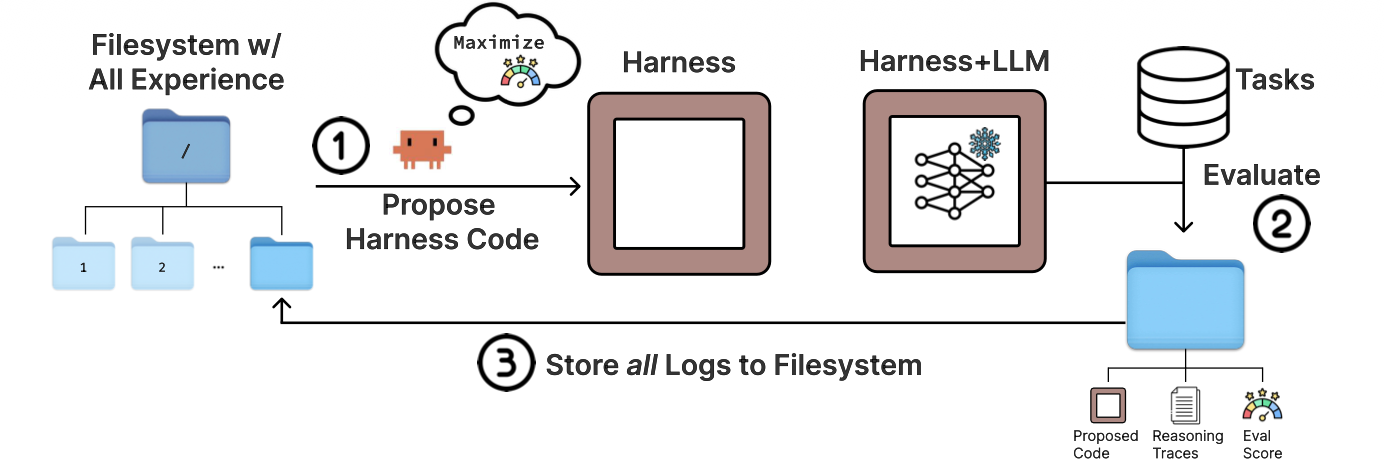
\includegraphics[width=\linewidth]{figures/metaharness.png}
    \caption{Illustration of the Meta Harness approach \citep{lee2026meta}}
    \label{fig:metaharness}
\end{figure}

Meta harness \citep{lee2026meta}  also achieves good results, using external memory and text optimization. Figure~\ref{fig:metaharness} illustrates how meta harness works. (1) A filesystem has all prior
candidates’ source code, execution traces, and scores; the agent reads this, and generates code for a new harness. (2) The proposed harness is evaluated on evaluation tasks. (3) All proposed code, reasoning
traces, and evaluation scores are stored in the filesystem in a new directory, and the loop repeats.

Self harness \citep{zhang2026self} and Agentic Harness Engineering \citep{lin2026agentic} further explore harness design, achieving substantial improvements on software engineering tasks. Recursive self-evolving agents \citep{nguyen2026recursive} focuses on the selection aspect of self-improving agents. 

Another use case is described by \citet{luo2026autodesign}. They  use a meta harness to design a harness for turning a scientific paper into a conference-poster. This work thus has contributions on two levels: a method for making a meta-harness, and a concrete harness for designing posters---which the authors, obviously, use on their own paper. 

\begin{figure}
    \centering
    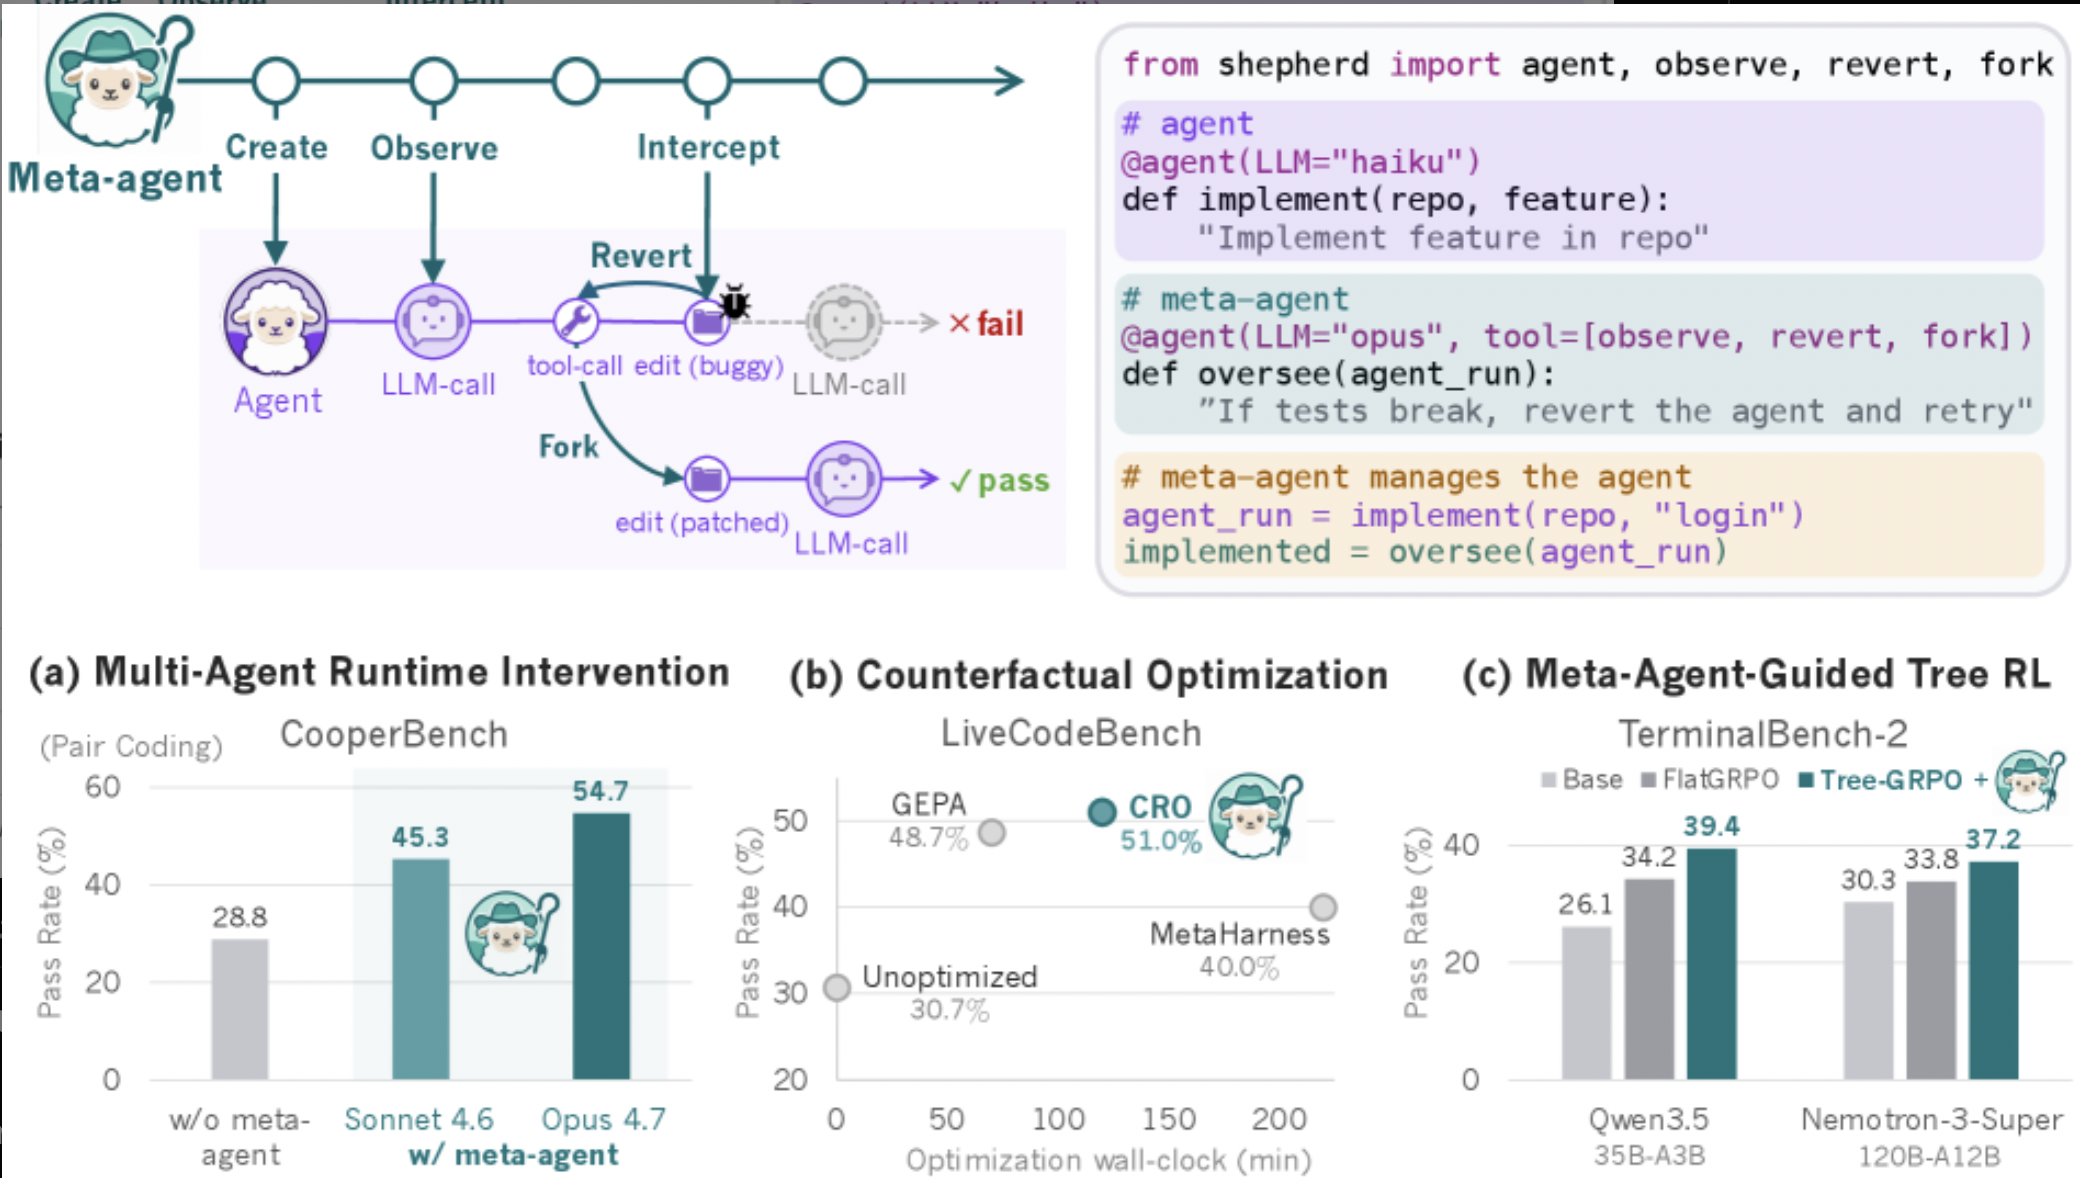
\includegraphics[width=\linewidth]{figures/shepherd.png}
    \caption{Illustration of the Shepherd Meta Agent Environment \citep{yu2026shepherd}}
    \label{fig:shepherd}
\end{figure}

The Shepherd system \citep{yu2026shepherd} provides a functional meta agent programming environment.\footnote{\url{https://shepherd-agents.ai}} Shepherd defines LLM agents as Python functions, allowing an agent's execution traces to be monitored, rolled-back, forked, modified, and resumed.  Early experiments show significant performance improvements on three different benchmarks, as illustrated in Figure~\ref{fig:shepherd}.

A comprehensive survey with more approaches on self-improving agent designs is \citet{ren2026self}. Their taxonomy explicitly recognizes the two-level architecture.

\section{Concluding Remarks}
In this chapter we have discussed some advanced architectures,  at the level of the transformers, and at the level of the agents. Both are highly active fields of research.

\bibliographystyle{plainnat}
\bibliography{agenticbook,refs,case,synthetic}
